\documentclass[10pt]{beamer}
\usepackage{amsmath}
\usepackage{amssymb}
\usepackage{geometry}
\usepackage{graphicx}
\usepackage{url}
\usepackage{bm}

\begin{document}

\begin{frame}
\large Lecture 15:\\ 
Inference for Simple Linear Regression\\
STAT 630, Fall 2021
\end{frame}

%-------------------------------------------
\begin{frame}{Inference for SLR}
\vspace{-2cm}
\textbf{Simple linear regression model for the population}:\\
$$ y_i = \beta_0 + \beta_1 x_i + \epsilon_i $$\\
$\beta_0$ and $\beta_1$ are the population parameters (fixed and non-random)
\vspace{15pt}

\textbf{Least squares line (estimated from the sample)}:\\
$$ \hat{y}_i = \hat{\beta}_0 + \hat{\beta}_1 x_i $$\\
$\hat{\beta}_0$ and $\hat{\beta}_1$ are the estimates (random, varies from sample to sample)
\end{frame}

%-------------------------------------------
\begin{frame}{Inference for SLR}
Test whether the slope $\beta_1$ is zero (i.e., whether there is a linear association between $x$ and $y$).\\
\vspace{10pt}
$H_0: \beta_1 = 0$\\
$H_A: \beta_1 \neq 0$\\
\vspace{10pt}
Test statistic:
$$t = \frac{\hat{\beta}_1}{se(\hat{\beta}_1)}; \quad \text{df=n-2}$$
\vspace{15pt}

$1-\alpha$ confidence interval for the slope $\beta_1$:
\begin{align*}
\hat{\beta}_1 \pm t_{\alpha/2; n-2} se(\hat{\beta}_1)
\end{align*}
\end{frame}


%-------------------------------------------
\begin{frame}{Inference for SLR}
Test whether the intercept $\beta_0$ is zero.\\
\vspace{10pt}
$H_0: \beta_0 = 0$\\
$H_A: \beta_0 \neq 0$\\
\vspace{10pt}
Test statistic:
$$t = \frac{\hat{\beta}_0}{se(\hat{\beta}_0)}; \quad \text{df=n-2}$$
\vspace{15pt}

$1-\alpha$ confidence interval for the intercept $\beta_0$:
\begin{align*}
\hat{\beta}_0 \pm t_{\alpha/2; n-2} se(\hat{\beta}_0)
\end{align*}
\end{frame}

%-------------------------------------------
\begin{frame}
Formulas for standard error computations (can use software for these computations):\\
\vspace{5pt}

\begin{itemize}
\item Residual standard error:
\begin{align*}
\hat{\sigma} = \sqrt{\frac{\sum_{i=1}^n \hat{e}_i^2}{n-2}} = \sqrt{\frac{\sum_{i=1}^n (y_i - \hat{y}_i)^2}{n-2}}
\end{align*}
\item Standard error of $\hat{\beta}_1$:
\begin{align*}
se(\hat{\beta}_1) = \frac{\hat{\sigma}}{\sqrt{\sum_{i=1}^n (x_i - \bar{x})^2}}
\end{align*}
\item Standard error of $\hat{\beta}_0$:
\begin{align*}
se(\hat{\beta}_0) = \hat{\sigma} \sqrt{\frac{1}{n} + \frac{\bar{x}^2}{\sum_{i=1}^n (x_i - \bar{x})^2}}\\
\end{align*}
\end{itemize}
\end{frame}

%-------------------------------------------
\begin{frame}[fragile]{Example}
Going back to the example of fitting a simple linear regression model for highway mileage, using weight as a predictor.
\begin{verbatim}
> library(MASS)
> lm1 <- lm(MPG.highway ~ Weight, data=Cars93)
> summary(lm1)

Coefficients:
              Estimate Std. Error t value Pr(>|t|)    
(Intercept) 51.6013654  1.7355498   29.73   <2e-16 ***
Weight      -0.0073271  0.0005548  -13.21   <2e-16 ***
---
Signif. codes:  0 ‘***’ 0.001 ‘**’ 0.01 ‘*’ 0.05 ‘.’ 0.1 ‘ ’ 1
\end{verbatim}
\begin{verbatim}

\end{verbatim}
\end{frame}

\begin{frame}{Example}
\vspace{-3.5cm}
(a) Do the data provide strong evidence of an association between weight and highway MPG?  State the null and alternative hypothesis, report the test statistic and $p$-value (from the \texttt{summary()} command), and state your conclusion.\\
% \vspace{11pt}
% 
% {\color{blue}
% $H_0: \beta_1 = 0$\\
% $H_A: \beta_1 \neq 0$\\
% \vspace{11pt}
% 
% Test statistic: $t = -13.21$
% \smallskip
% 
% Since the $p$-value $< \texttt{2e-16} \approx 0$, we reject $H_0$. The data provide strong evidence of a linear association between car weight and highway MPG.
% }

\end{frame}

\begin{frame}{Example}
\vspace{-3.5cm}
(b) Calculate a 95\% confidence interval for the slope $\beta_1$.  Note that there are $n=93$ car models (rows) in the data set.\\
% \vspace{11pt}
% 
% {\color{blue}
% \texttt{qt(0.975, df = 91) = 1.986}
% \begin{align*}
% \hat{\beta}_1 \pm t_{\alpha/2; n-2} se(\hat{\beta}_1)
% &\implies -0.0073 \pm 1.986 (0.00055)\\
% &\implies (-0.0084, -0.0064)
% \end{align*}}

\end{frame}

\begin{frame}{Example}
\vspace{-3.5cm}
(c) For the intercept term, the output from \texttt{summary()} gives a test statistic $t=29.73$ and $p$-value \texttt{< 2e-16}.  What are the null and alternative hypotheses that are being tested?  What is the conclusion of the test?
% \vspace{11pt}
% 
% {\color{blue}
% $H_0: \beta_0 = 0$\\
% $H_A: \beta_0 \neq 0$\\
% \vspace{11pt}
% 
% Since the $p$-value $\approx 0$, we reject $H_0$.  The intercept $\beta_0$ is significantly different than 0.\\ 
% }
\end{frame}

%-------------------------------------------
\begin{frame}{Conditions for SLR}
\begin{itemize}
\item \textbf{Linearity}.  The data should follow a linear trend.
\vspace{5pt}
\item \textbf{Constant variability}.  The variability of points around the least squares line remains roughly constant.
\vspace{5pt}
\item \textbf{Normality}.  The residuals should be approximately normally distributed with mean 0.
\vspace{5pt}
\item \textbf{Independence}.  Values of the response variable are independent of each other. 
\end{itemize}
\end{frame}

%-------------------------------------------
\begin{frame}{Residual Plots}
\begin{itemize}
\item One useful way to check the conditions is to look at a plot of the residuals $\hat{e}_i = y_i - \hat{y}_i$ versus $x_i$ for $i=1, \cdots, n$.  It is also common to plot the residuals $\hat{e}_i$ versus the fitted values $\hat{y}_i$ (for simple linear regression the plots look the same).
\vspace{5pt}
\item One purpose of residual plots is to identify characteristics or patterns still apparent in the data after fitting the model.
\vspace{5pt}
\item Residual plots are especially useful for checking linearity and constant variability.
\vspace{5pt}
\item Ideally, the residual plot should show no obvious pattern, and the points are randomly scattered around 0.
\end{itemize}
\end{frame}

%-------------------------------------------
\begin{frame}{Example: Residual Plot}
For the simple linear regression model between car weight and highway mileage, the points in the residual plot look randomly scattered and show no obvious patterns, except for slight nonconstant variability, indicating that the conditions are reasonably satisfied.

\centering
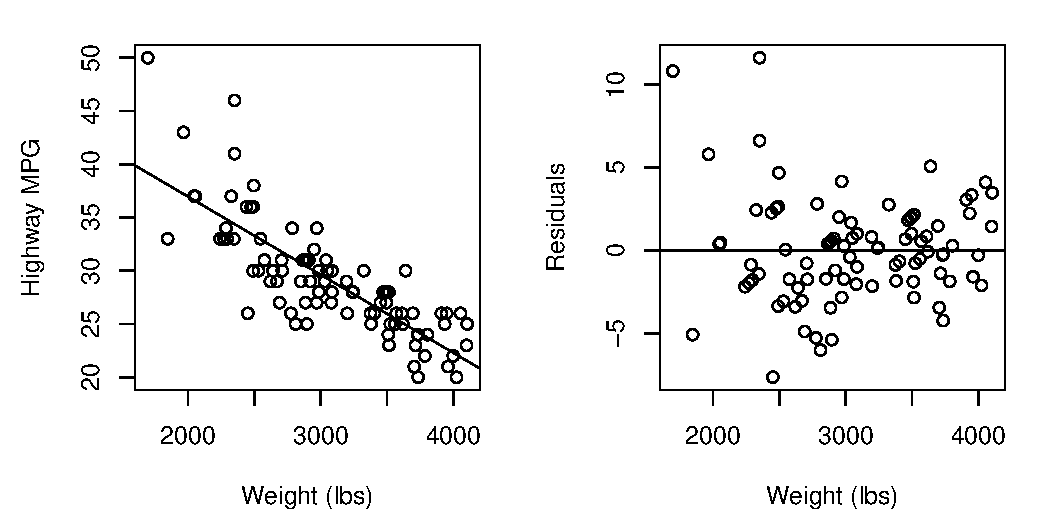
\includegraphics[scale=0.6]{figure/mpg_lmplots.pdf}
\end{frame}

%-------------------------------------------
\begin{frame}[fragile]
Here is the code used to create the last plot.
\begin{verbatim}
library(MASS)

# fit linear model
lm1 <- lm(MPG.highway ~ Weight, data=Cars93)

# scatter plot with least squares line
> plot(Cars93$Weight, Cars93$MPG.highway, 
       xlab = "Weight (lbs)", ylab = "Highway MPG")
> abline(lm1)

# residual plot
> plot(Cars93$Weight, resid(lm1),
       xlab = "Weight (lbs)", ylab = "Residuals")
> abline(h=0)
\end{verbatim}
\end{frame}

%-------------------------------------------
\begin{frame}[fragile]{Example: Normality of Residuals}
To check whether the residuals follow a normal distribution, make a histogram and QQ plot.  For the example below, the residuals look normally distributed, except for two potential outliers.

\small
\begin{verbatim}
> par(mfrow=c(1,2)) 
> hist(resid(lm1), xlab = "Residuals", main= "")
> qqnorm(resid(lm1))
> qqline(resid(lm1))
\end{verbatim}

\centering
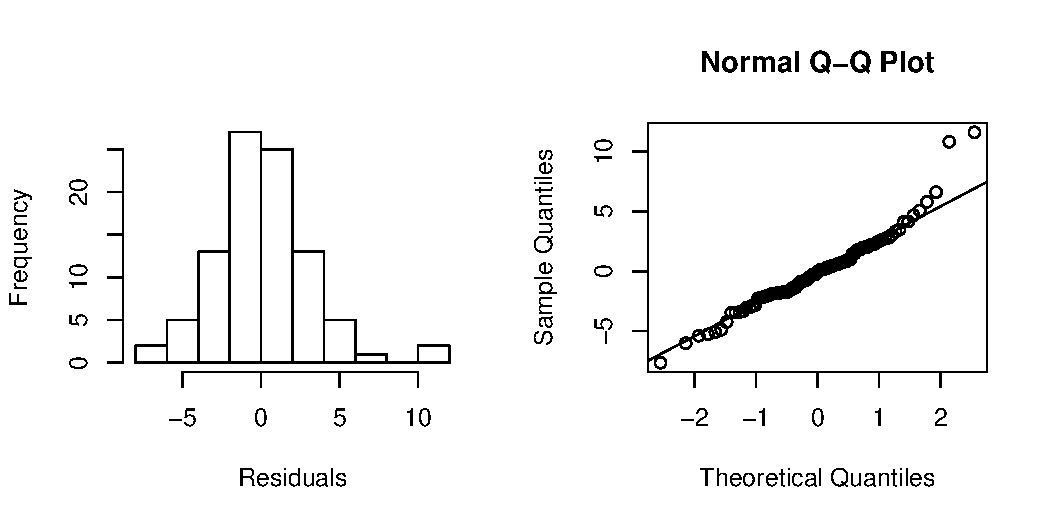
\includegraphics[scale=0.55]{figure/cars_norm_resid.pdf}
\end{frame}


%-------------------------------------------
\begin{frame}{Example: Nonconstant Variability}
An example of a violation of the constant variability condition.  The residual plot shows a fan pattern.  This is sometimes called \textbf{heteroscedasticity}.
%In the scatter plot between $x$ in $y$ we can also see that as $x$ increases the varability in the points around the line increases.

\centering
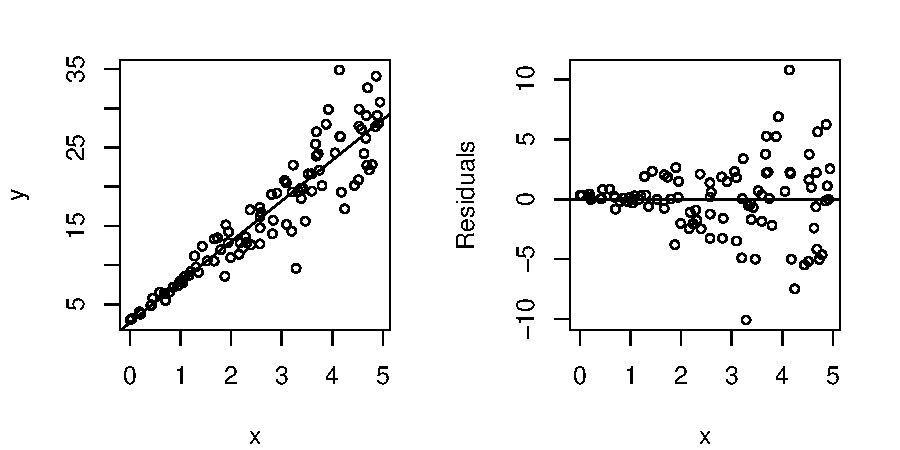
\includegraphics[scale=0.6]{figure/resid_var.pdf}
\end{frame}

%-------------------------------------------
\begin{frame}{Example: Nonlinearity}
An example of a violation of the linearity condition.

\centering
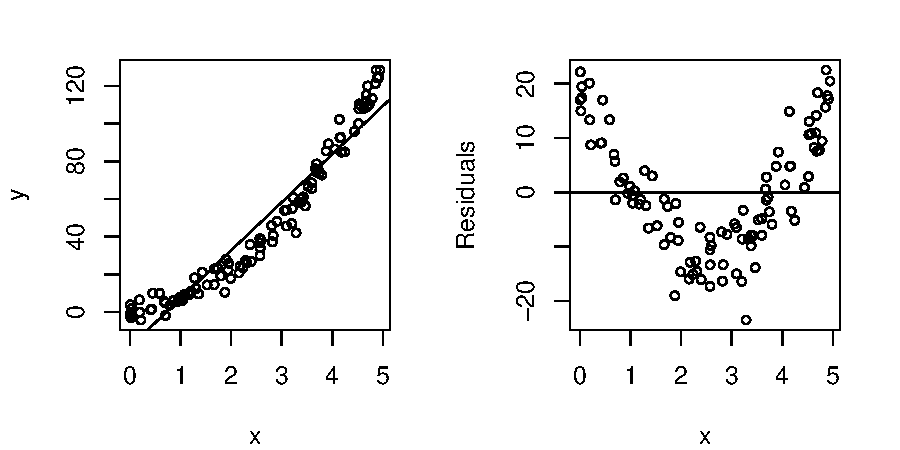
\includegraphics[scale=0.6]{figure/resid_nonlin.pdf}
\end{frame}


\end{document}